\label{timeline}
Given the size of the problem space and that the proposed work will be performed in no more than nine month, we propose to focus on three main contributions:
\begin{inparaenum}[(1)]
\item evaluating and deriving the makespan for a campaign as a set of independent static O(10) workflows with heterogeneous resource requirements provided by ecological and biomolecular sciences use cases on dynamic resources; 
\item offering execution planning capabilities to minimize the makespan of a campaign; and 
\item validating our planning capability by executing the workflows of our use cases and measuring the accuracy of the estimated campaign runtime and planned execution compared to a random plan.
\end{inparaenum}.
In addition, we will explore the requirements to support campaigns with dynamic workflows.

To this end, we propose to achieve the following objectives with an estimation of the time needed:
\begin{enumerate}
    \item Develop a campaign manager prototype, which will derive and execute a plan. Duration 3 months
    \item Implement proposed makespan algorithm for executing a campaign from the ecological sciences. Duration 3 months.
    \item Experimentally measure the performance of the selected makespan algorithm for a scientific campaign. Duration 5.5 months. It overlaps with objective 2 
\end{enumerate}
Figure~\ref{fig:work_plan} shows the Gantt chart of the proposed work.

\begin{figure*}[t]
	\centering
	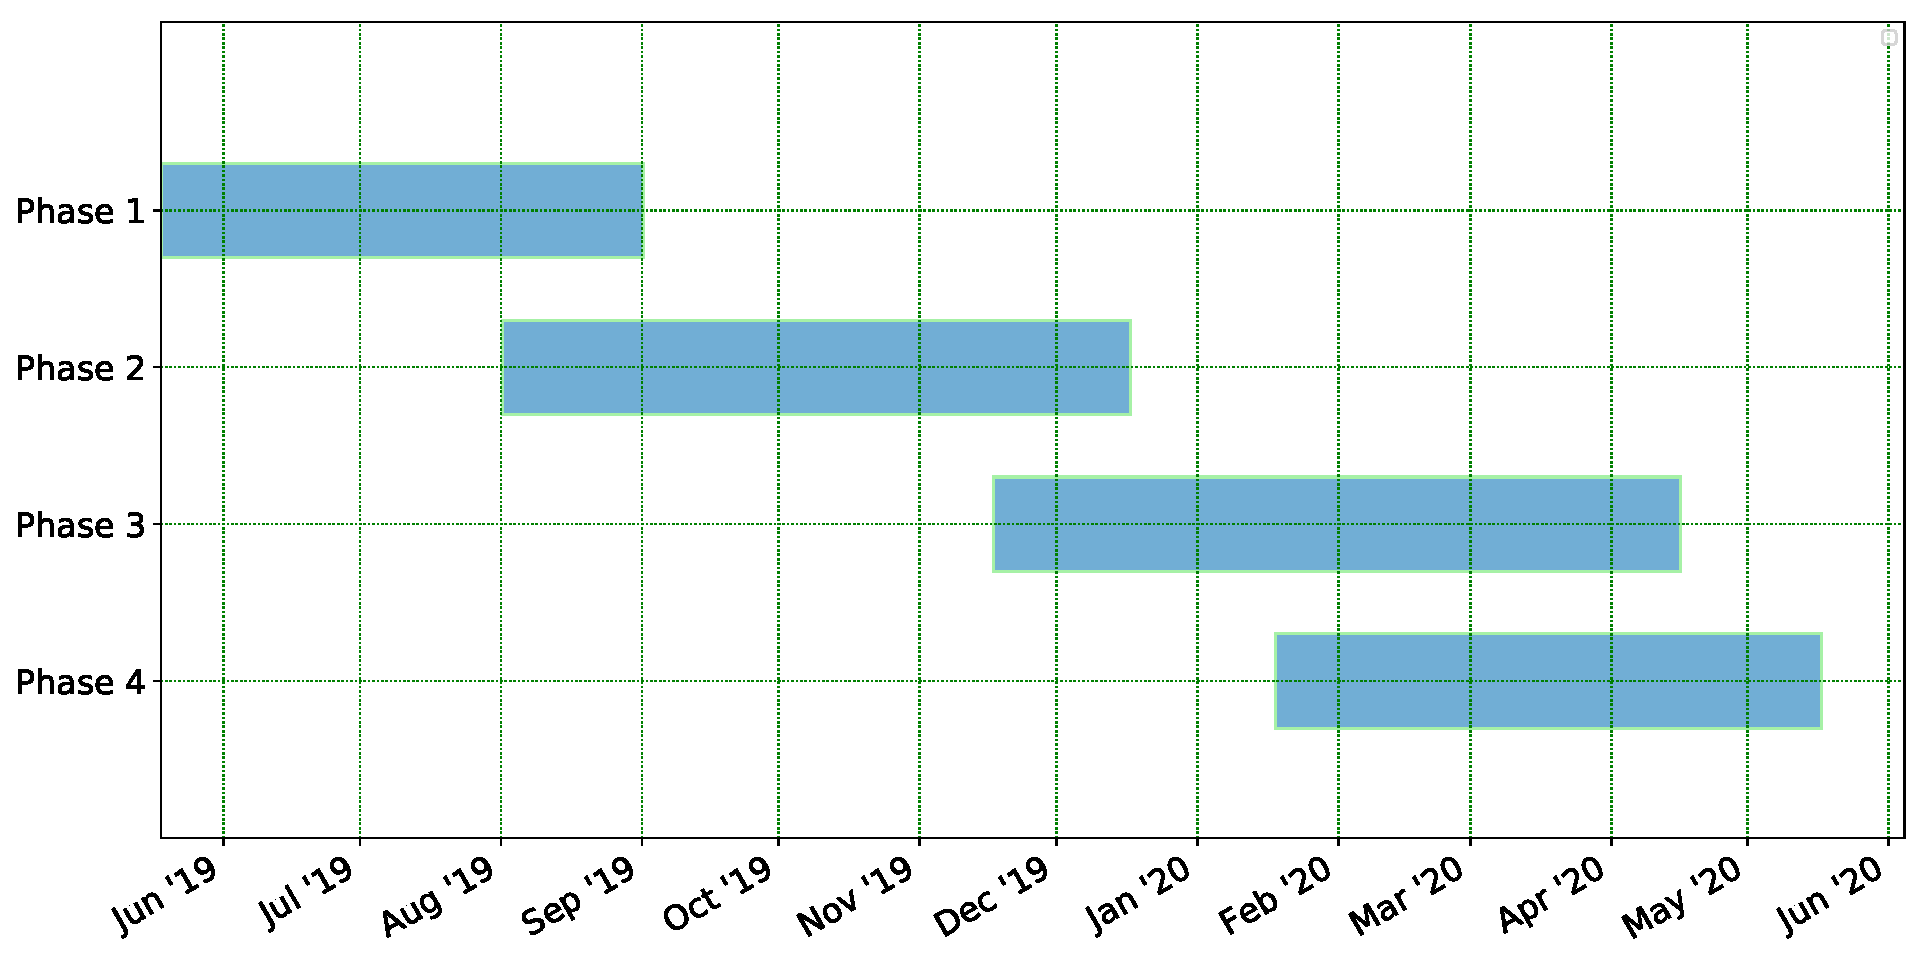
\includegraphics[width=.95\textwidth]{figures/phd_plan.pdf}
	\caption{Planned timeline of proposed research}\label{fig:work_plan}
\end{figure*}

\subsubsection{Phase 1: Design and implementation of a campaign manager}
Phase 1 would include design discussions for a prototype of the campaign manager.
Design a prototype is an iterative process, and it will provided the basic functionality of the campaign manager.
Result of these discussions will be the requirements of the campaign manager and its API. 
Design will be finalized and a prototypical implementation will be completed by Month 3. 
The prototype will interface with RADICAL-EnTK providing campaign execution capabilities.

\subsubsection{Phase 2: Implementation and performance analysis of makespan algorithm}
Phase 2 includes implementing the proposed algorithm in the prototype, supporting dynamic resources and understand its performance.
In case the selected algorithm under performs, a study will be conducted with additional makespan algorithms.
Phase 2 spans from months 3 up to 6.

\subsubsection{Phase 3: Experimental performance analysis}
Phase 3 of the plan includes an experimental performance analysis of the campaign manager for a set of selected use cases.
This performance analysis will compare the execution a computational campaign with the prototypical campaign manager and without.
This phase span between months 3 and 9.

% ---------------------------------------------------------------------------
% Why
\subsection{Significance and impact of work}
Several scientific campaigns require to execute a large number of workflows several times with different input data or initial conditions. 
The required concurrency to minimize the execution time of the campaign is not necessarily constant and may change based on resource availability. 
The campaign manager suggested in this proposal will be the first to make resource selection decisions for the users. 
This will lead to less time invested by users to make execution decisions about their workflows. 
These decisions will lead to better resource utilization and, as a result, better domain science. 
The empirical performance analysis derived by this work can be used to derive empirical models initial and eventually formal mathematical models.

% ---------------------------------------------------------------------------
% Challenges
\subsection{Challenges/Risks}

We estimate the proposed work, divided into three major phases, to take 9 months 
and we allocate 3 months to account for unforeseen circumstances. We would like 
to keep the committee aware of the following challenges that we see:

\begin{itemize}
	\item Design and Implementation (phase 1) is iterative and special attention needs to be given to the number of iterations against specific objectives, given the timeline.
    \item All experiments performed on HPC systems are subject to variable queue times and may limit the number of experiments performed in phase 2 and 3.
	\item Although the middleware will be well tested (80--90\% of the code base will be covered by unit tests) and less susceptible to major changes, RADICAL-Pilot is known to be less stable and is susceptible to changes as it serves multiple projects. Stability of RADICAL-Pilot is considered in the estimates, but needs to be made aware to the committee.
\end{itemize}